%%------------------------------------------------------
%  
%  Testing include for dissertation
%
%------------------------------------------------------

\section{ Unit Testing }

At the beginning of the project, Unit tests for Patridge's server and paper
preprocessing components were written in order to test that the main bulk of
the application worked before it was deployed to the production system at
\url{http://farnsworth.papro.org.uk}. These tests were written and maintained
throughout the project and occasionally had to be changed as code was
refactored. As each new feature was added to the system, the whole suite of
tests was executed to provide integration coverage and make sure that new
features did not break existing code. 

\subsection{ Backend \& Infrastructure Testing}

The backend of the system was tested using Python unit tests based upon the
built in \emph{unittest} module and a third party testing library called
\emph{Nose} which provided automated test discovery. This meant that a user who
ran the command \emph{nose} from the project directory could automatically find
and run all of the unit tests in the project without having to set up
boilerplate test suites as in \emph{JUnit}.



\subsection{ Selenium \& Frontend Testing }

The frontend parts of Partridge that were written in Javascript and HTML5 also
had to be tested to verify that the query and upload forms behaved as expected.


\section{ User Testing } 

Once a basic user interface had been implemented, the system was opened for
user testing. The main Patridge instance
(\url{http://farnsworth.papro.org.uk/}) was advertised using several social
media streams and users encouraged to submit bug reports if they experienced
any problems whilst using the site.


\section{ Evaluating Learning Algorithms }

As discussed above, Patridge uses a supervised learning algorithm, a Random
Decision Forest, to classify the type of each of the scientific papers added to
its database. Unlike traditional procedural algorithms that can be unit tested
and in some cases formally proven to behave uniformly at
runtime\cite{filliatre2007formal}, supervised learning algorithms are imperfect
systems that build `working models' from known data. This makes the performance
of supervised learning systems much more difficult to assess. Russell and
Norvig(2010) suggest that ``a learning system is good if it produces hypotheses
that do a good job of predicting the classification of unseen
examples\cite{russell2010artificial}." It is suggested that when training a
supervised learning system, some of the example data should be kept back when
during the training phase and instead, used as `unseen examples' and classified
by the newly trained system to judge its accuracy
\cite{alpaydin2004introduction}\cite{russell2010artificial}.

A common technique for partitioning data into `seen' and `unseen' or training
and test data sets is to simply split the data into two sets through the use of
random sampling.  A 60:40 divide between training and test data is common.
Witten explains that ``it is better to use more than half the data for
training, even at the expense of test data\cite{witten2005data}." 

\subsection{ Three Fold Validation }

Three fold validation is a commonly used method for using all of the available
data for both testing and training whilst still maintaining . As the name
suggests, test data is split into three disjoint sets and then the classifier
is trained on two of the sets and tested with the third. This is repeated three
times so that all sets are used for both training and testing. Results from
each of the folds can be represented separately or an average taken.

\subsection{ Result Presentation } 

Results from the evaluation methods discussed above can be presented in a
number of ways. When working with machine learning systems, it is important to
analyse performance using a selection of techniques in order to get a
comprehensive image of the capabilities and restrictions of the system.

Classifier Accuracy (CA), Receiver Operating Characteristics
(ROC) charts and Area Under the Curve (AUC) give a general overview of the
classifier's behaviour, whilst confusion matrices, recall, precision and
f-measure give a detailed view of which specific data types were most
frequently misclassified and what they were mistaken for. 

\subsubsection{ Classifier Accuracy } 

The CA of a supervised classifier is simply represented as the percentage of
the test data that the classifier was able to predict correctly. CA values that
tend towards 1.0 correspond to a more accurate classifier. In a Three Fold
validation, the CA for the classifier is calculated by taking the mean of the
individual performance values from each of the test/train cycles. 

3 Fold Validation on the Partridge corpus  

\subsubsection{ Receiver Operating Characteristics Chart}

Receiver Operating Characteristics (ROC) Charts are used to visually represent
the trade-off between True Positives(TP) and False Positives(FP) as identified
by the classifier under evaluation. Witten(2005) explains that ROC is a method
reappropriated from signal processing analysts who use it to visualise ``...hit
rate and false alarm rate over noisy communication
channels\cite{witten2005data}." The ratio of TP to FP classifications is
measured with increasing numbers of test samples from left to right. 

ROC charts are often divided into halves diagonally by a line indicating where
the TP-FP ratio is equal. There may be multiple plots on the axes if several
learning algorithms are under evaluation. A graph plot that presents a steep
curve that mostly fits into the upper left half of the graph shows a high TP-FP
ratio which is a sign that the classifier is working well.  Figure
\ref{fig:roc_random_forest} shows the ROC Chart for Partridge's Topic
Classifier after training on 60\% of the Partridge corpus and testing on 40\%.

\begin{figure}[!h]
\begin{center}
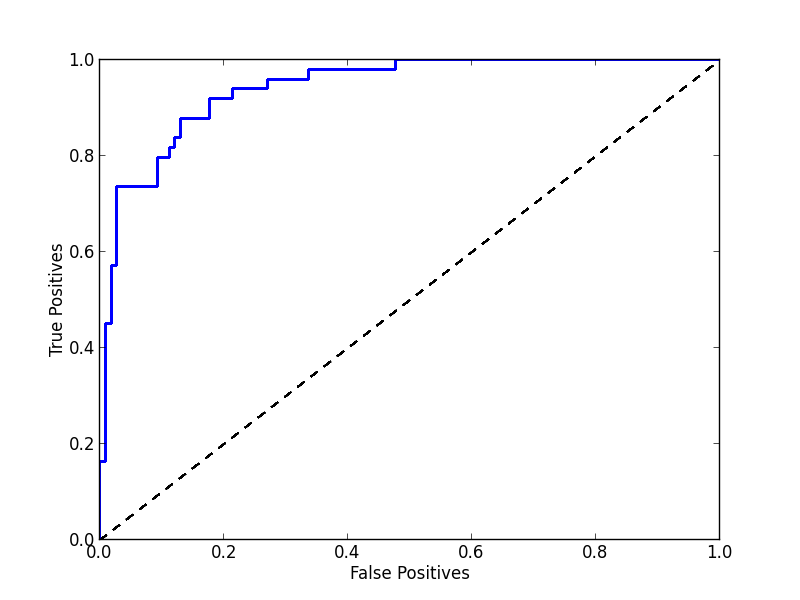
\includegraphics[width=0.65\textwidth]{images/testing/ROC.png}
\caption{ ROC Curve for Partridge's Random Forest Topic Classifier}
\label{fig:roc_random_forest}
\end{center}
\end{figure}

\subsubsection{ Area Under Curve }

The Area Under the Curve (AUC) measure is calculated as a percentage of  the
area underneath a ROC curve. This can again be used to give an indication of
the trade-off between true positive and false positive classification. It is a
percentage measurement, where 100\% indicates a high TP-FP ratio. AUC is often
used instead of visualising a ROC graph for brevity or where average
performance of a classifier over several train-test cycles is to be calculated.
The average AUC for Partridge's Random Tree Paper Type classifier after is
96.6\% after three fold validation is executed over the whole set of papers.

Comparison of this result with the above graph does show discrepancies between
simple 60:40 proportional validation and 3-fold validation - the average
performance of the latter seems to be slightly more accurate. This may be
because a slightly higher number of training examples (66\% rather than 60\%)
were used to train the classifiers during 3-fold validation and that the errors
were averaged out at the end of the process.

\subsubsection{ Confusion Matrices}

Confusion Matrices are a way of showing comprehensively which classes a machine
learning system struggles to discriminate between the most. Known classes are
shown on the vertical axis of the matrix and predicted classes are shown across
the horizontal. This allows inference of which data classes a trained
classifier struggles to label most frequently and any classes that it commonly
confuses them with. A set of confusion matrices for the Paper Type Classifier
in Partridge can be seen in Figure \ref{fig:conf_matrices} below.

\begin{figure}[!h]

\centering

\begin{subfigure}[b]{\textwidth}

\caption{Fold 1 Results}
\centering
\begin{tabular}{| l || l | l | l |}
\hline
	&	Case Study&	Research&	Review\\
\hline
\hline
Case Study&	83&		2&		12\\
\hline
Research&	3&		255&		0\\
\hline
Review&		4&		2&		159\\
\hline

\end{tabular}
\end{subfigure}


\begin{subfigure}[b]{\textwidth}

\caption{Fold 2 Results}
\centering
\begin{tabular}{| l || l | l | l |}
\hline
&	        Case Study&     Research&	Review\\
\hline
\hline
Case Study&     85    &         2&		10\\
\hline
Research&	0   &		256&		2\\
\hline
Review&		5&		1&		159\\
\hline
\end{tabular}

\end{subfigure}

\begin{subfigure}[b]{\textwidth}

\caption{Fold 3 Results}
\centering
\begin{tabular}{| l || l | l | l |}
\hline
&		Case Study&	Research&	Review\\
\hline
\hline
Case Study&	82&		3	&	12 \\
Research&	0&		257	&	1\\
Review&		7&		2	&	156\\
\hline
\end{tabular}

\end{subfigure}

\caption{ Confusion matricies for the 3-Fold validation process}
\label{fig:conf_matrices}

\end{figure}

These results show that Partridge's decision tree is very effective at
classifying the three document types in its database. It is also clear however,
that whilst the classifier is outstanding at recognising Research papers, it
sometimes struggles to discriminate between Case Study and review papers. This
may be because case studies can be considered a specific type of review paper
and the two classes share more similar CoreSC features than they do with
research papers.  

\subsubsection{ Precision, Recall and F-Measure }

From a classifier's confusion matrices, it is possible to calculate its
Precision, Recall and F-Measure values. These can be used to make further
assertions about the validity of a classifier's behaviour
\cite{witten2005data}.

The Precision of a classifier is the fraction of data samples retrieved that
were correctly classified. This is defined as:
\[Precision = \frac{tp}{tp+fp} \]

The Recall of a classifier is the proportion of samples within a given class
that the classifier is able to correctly classify. For example: the number of
apples that a classifier identifies as apples within a training set of fruit.
This is defined as:
\[Recall = \frac{tp}{tp+fn} \]

The F-Measure of a classifier is used to characterise both Recall and Precision
in a single value. The F-Measure of a classifer can be defined as:
\[
F-Measure = \frac{ 2 \times Recall \times Precision} { Recall + Precision } = 
\frac{2 . TP}{ 2 . TP + FP + FN }
\]


\begin{figure}[!th]

\centering
\begin{tabular}{| l | l | l | l | l |}
\hline
&        &\textbf{Recall}&\textbf{Precision}&\textbf{F-Measure}\\
\hline
\hline
\multirow{4}{*}{Fold 1} & Case Study & 0.85 & 0.92 & 0.89 \\
                        & Review     & 0.96 & 0.92 & 0.94 \\
                        & Research   & 0.98 & 0.98 & 0.98 \\
\hline

\multirow{4}{*}{Fold 2} & Case Study & 0.87 & 0.94 & 0.91 \\
                        & Review     & 0.96 & 0.92 & 0.94 \\
                        & Research   & 0.99 & 0.98 & 0.99 \\

\hline

\multirow{4}{*}{Fold 3} &Case Study & 0.84 & 0.92 & 0.88 \\
                        & Review    & 0.95 & 0.92 & 0.93 \\
                        & Research  & 0.99 & 0.98 & 0.99 \\


\hline


\end{tabular}

\caption{Recall Precision and F-Measure values for Partridge Topic Classifier}
\label{fig:fmeasure_table}

\end{figure}

Recall, Precision and F-Measure was calculated for each of the classes and in
each iteration of the three fold validation sequence. The results in Figure
\ref{fig:fmeasure_table} show good recall, precision and f-measure for all
three document types within Partridge. These results verify that Case Study is
the hardest document type to classify as discussed above.

